%File: formatting-instruction.tex
\documentclass[letterpaper]{article}
\usepackage{aaai}
\usepackage{times}
\usepackage{helvet}
\usepackage{courier}
\usepackage{graphicx}
\usepackage{amssymb}
\usepackage{amsmath}
\usepackage{amssymb}
\usepackage{color}
\usepackage{tikz}
\usepackage{pgfplots}
\usepackage{caption}
\usepackage{subcaption}
\usepackage{comment}
\usepackage{booktabs}
\usepackage{nopageno}
\usepackage{url}
\usepackage{chessboard}
\usepackage{skak}

\usepackage[algo2e, noend, noline, linesnumbered]{algorithm2e}
\providecommand{\SetAlgoLined}{\SetLine}  
\providecommand{\DontPrintSemicolon}{\dontprintsemicolon}
\DontPrintSemicolon
\makeatletter
\newcommand{\pushline}{\Indp}% Indent
\newcommand{\popline}{\Indm}
\makeatother
\newcommand{\argmax}{\operatornamewithlimits{argmax}}
\newcommand{\defword}[1]{\textbf{\boldmath{#1}}}

\captionsetup{compatibility=false}

%\pgfplotsset{compat=newest}
\usetikzlibrary{arrows,shapes,petri}

\newcommand{\bE}{\mathbb{E}}
\newcommand{\bQ}{\bar{Q}}
\newcommand{\cA}{\mathcal{A}}
\newcommand{\cC}{\mathcal{C}}
\newcommand{\cD}{\mathcal{D}}
\newcommand{\cG}{\mathcal{G}}
\newcommand{\cI}{\mathcal{I}}
\newcommand{\cN}{\mathcal{N}}
\newcommand{\cO}{\mathcal{O}}
\newcommand{\cR}{\mathcal{R}}
\newcommand{\cS}{\mathcal{S}}
\newcommand{\cT}{\mathcal{T}}
\newcommand{\cZ}{\mathcal{Z}}
\newcommand{\hQ}{\hat{Q}}
\newcommand{\hV}{\hat{V}}
\newcommand{\eg}{{\it e.g.,}~}
\newcommand{\ie}{{\it i.e.,}~}

% the note center!
\definecolor{darkgreen}{RGB}{0,125,0}
\newcounter{nsNoteCounter}
\newcounter{mlNoteCounter}
\newcounter{mwNoteCounter}
\newcounter{tpNoteCounter}
\newcommand{\nsnote}[1]{{\scriptsize \color{blue} $\blacksquare$ \refstepcounter{vlNoteCounter}\textsf{[NS]$_{\arabic{vlNoteCounter}}$:{#1}}}}
\newcommand{\mlnote}[1]{{\scriptsize \color{darkgreen} $\blacksquare$ \refstepcounter{mlNoteCounter}\textsf{[ML]$_{\arabic{mlNoteCounter}}$:{#1}}}}
\newcommand{\mwnote}[1]{{\scriptsize \color{red} $\blacktriangle$ \refstepcounter{asNoteCounter}\textsf{[AS]$_{\arabic{asNoteCounter}}$:{#1}}}}
\newcommand{\tpnote}[1]{{\scriptsize \color{orange} $\blacktriangle$ \refstepcounter{asNoteCounter}\textsf{[TP]$_{\arabic{asNoteCounter}}$:{#1}}}}
%\newcounter{NoteCounter}
%\newcommand{\vlnote}[1]{{\scriptsize \color{blue} \refstepcounter{vlNoteCounter}\textsf{[VL]$_{\arabic{vlNoteCounter}}$:{#1}}}}
%\renewcommand{\vlnote}[1]{}


\frenchspacing
\setlength{\pdfpagewidth}{8.5in}
\setlength{\pdfpageheight}{11in}
\pdfinfo{
/Title (Insert Your Title Here)
/Author (Put All Your Authors Here, Separated by Commas)}
\setcounter{secnumdepth}{0}  

\begin{document}
% The file aaai.sty is the style file for AAAI Press 
% proceedings, working notes, and technical reports.
%
\title{Monte Carlo Tree Search with Heuristic Evaluations\\using Implicit Minimax Backups}
\author{Authors}

\maketitle

\begin{abstract}
Monte Carlo Tree Search (MCTS) has improved the performance of game-playing engines in 
domains such as Go, Hex, and general-game playing. MCTS has been shown to outperform 
classic minimax search in games where good heuristic evaluations are difficult to obtain. 
In recent years, combining 
ideas from traditional minimax search in MCTS has been shown to be advantageous in some domains,
such as Lines of Action, Amazons, Breakthrough, Connect Four, and Kalah. In this paper, we propose 
a new way to use heuristic evaluations to guide the MCTS search by storing the two sources of 
information, estimated win rates and heuristic evaluations, separately. 
Rather than using the heuristic evaluations to replace the playouts, 
our technique backs them up {\it implicity} during its MCTS simulations. 
These learned evaluation values are then used to guide future simulations. 
Compared to current techniques, we show that using implicit minimax backups  
reduces regret in an example game and leads to stronger 
play performance in Breakthrough, Lines of Action, and Kalah, (...and Hearts?).
\end{abstract}

%\subsection{Related Work}

\section{Introduction}

Monte Carlo Tree Search (MCTS)~\cite{Coulom06Efficient,Kocsis06Bandit} is a simulation-based best-first
search paradigm that has been shown to increase performane in domains such as turn-taking games, 
general-game playing, real-time strategy games, single-agent planning, and more~\cite{mctssurvey}. 
While the initial applications have been to games where heursitic evaluations are difficult to obtain, 
progress in MCTS research has shown that heuristics can be effectively be combined in MCTS, even in games 
where class minimax search has traditonally been preferred. 

The most popular Monte Carlo tree search algorithm is UCT~\cite{Kocsis06Bandit}, an algorithm
which performs a single simulation from the root of the search tree to a terminal state at each iteration. 
During the iterative process, a model of the game tree is incrementally built by adding a 
new leaf node to the tree on each iteration. 
The nodes in the tree are used to store statistical information regarding wins and losses, and backpropagation
policies are used to update parent estimates, and these improving estimates are then used to guide future simulations. 
When the simulation reaches parts of the game tree not included in the model, a default playout policy
is used to simulate to a terminal state where a win or loss is determined. 

%When applied to sequential turn-taking games, MCTS has primarily been used in domains where good 
%heuristic evaluations are difficult to obtain. 
In this work, we propose to augment MCTS with the help of 
an implicitly-computed minimax search which uses heuristic evaluations. 
Unlike previous work, these heuristic evaluations are used as {\it separate source of information}, 
and backed up in the same way as in classic minimax search. These minimax-style backups are done {\it implicitly}
as a simple extra step during the standard simulation, and always maintained separately from win rate estimates obtained
from playouts. These two separate information sources are then used to guide the MCTS search. 
We show that combining heuristic evaluations in this way reduces simple regret and improves performance in four 
different games. 

\subsection{Related Work}

Several techniques for minimax-influenced backup rules in the simulation-based MCTS framework have already been proposed. 
The first was Coulom's original {\it maximum backpropagation}~\cite{Coulom06Efficient}. This method of backpropagation
suggests, after a number of simulations to a node has been reached, to switch to propagating the maximum value instead 
of the simulated (average) value. 
The rationale behind this choice is that after a certain point, the search algorithm should consider the node
{\it converged} and return an estimate of the best value. 
Maximum backpropagation has also been used in other Monte Carlo tree search algorithms and demonstrated success in
probabilistic planning, as an alternative type of forecaster in BRUE~\cite{Feldman13Theoretically} and as Bellman 
backups for online dynamic programming in Trial-based Heuristic Tree Search~\cite{Keller13Trial}.

The first use of enhancing MCTS using prior knowledge was in Computer Go~\cite{Gelly07Combining}. 
In this work, offline-learned knowledge initialized values of expanded nodes increased performance against significantly against 
strong benchmark player. This technique was also confirmed to be advantageous in Breakthrough~\cite{Lorentz13Breakthrough}. 
Another way to introduce prior knowledge is a progressive bias during selection~\cite{Chaslot08Progressive}, which also showed 
increased performance in Go play strength. 

In games where minimax search performs well, such as Kalah, 
modifying MCTS to use minimax-style backups and heuristic values instead to replace playouts offers a worthwhile trade-off 
under different search time settings~\cite{Ramanujan11Tradeoffs}.
Similarly, there is further evidence suggesting not replacing the playout entirely, but terminating them early 
using heuristic evaluations, has increased the performance in Lines of Action (LOA)~\cite{Winands10MCTS-LOA}, 
Amazons~\cite{Kloetzer10Amazons,Lorentz08Amazons}, and Breakthrough~\cite{Lorentz13Breakthrough}. In LOA and Amazons, the 
MCTS players enhanced with evaluation functions outperform their minimax counterparts using the same evaluation function.

% mention score-bounded mcts
% mention hendrik's minimax methods
% use mcts-solver to motivate implicit minimax
%\marcl{Also mention MCTS + minimax hybrids (Baier \& Winands) and Score-bounded MCTS (...))}

One may want to combine minimax backups or searches without using an evaluation function. 
The prime example is MCTS-Solver~\cite{Winands08Solver}. When using 
MCTS-Solver, proven wins and losses are backpropagated as extra information in MCTS. When a node is proven to be a 
win or a loss, it no longer needs to be searched. This simple, domain-independent modification greatly enhances 
MCTS in many games (some examples). Score-bounded MCTS extends this idea to games with multiple outcomes, 
leading to $\alpha \beta$ style pruning in the tree~\cite{Cazenave10ScoreBounded}. Finally, one can use hybrid
minimax searches in the tree to initialize nodes during, enhance the playout, or to help MCTS-Solver 
in backpropagation~\cite{Baier13MinimaxHybrids}.

Finally, recent work has attempted to explain and identify some of the shortcomings that arise from estimates in 
MCTS, specifically compared to situations where classic minimax search has historically performed 
well~\cite{Ramanujan10Understanding,Ramanujan10On}. 
Attempts have been made to overcome the problem of {\it traps} or {\it optimistic moves} (strategic  
tactial lines that are problematic for MCTS) such as sufficiency thresholds during selection~\cite{Gudmindsson13Sufficiency} 
and shallow minimax searches~\cite{Baier13MinimaxHybrids}. We show that implicit minimax backups also
improve performance in domains with tactical short-term goals. 

\section{Adversarial Search in Turn-Taking Games}

%The following notation is taken from~\cite{Sutton98}

A finite deterministic Markov Decision Process (MDP) is 4-tuple $(\cS, \cA, \cT, \cR)$. Here, $\cS$ is a finite non-empty set of {\it states}. 
$\cA$ is a finite non-empty set of {\it actions}, where we denote $\cA(s) \subseteq \cA$ the set of available actions at state $s$. 
$\cT : \cS \times \cA \mapsto \Delta \cS$ is a {\it transition function} mapping 
each state and action to a distribution over successor states. Finally, $\cR : \cS \times \cA \times \cS \mapsto \Re$ 
is a {\it reward function} mapping (state, action, successor state) triplets to numerical rewards. 

A two-player perfect information game is an MDP with a specific form. 
Denote $\cZ = \{ s \in \cS: \cA(s) = \emptyset \} \subset \cS$ the set of {\it terminal states}. 
In addition, for all nonterminal states $s' \in \cS - \cZ$, $\cR(s,a,s') = 0$. 
There is a {\it player identity function} $\tau : \cS - \cZ \mapsto \{1,2\}$. 
In this paper, we assume fully deterministic domains, so $\cT(s,a)$ maps to a single state. 
When it is clear from the context and unless otherwise stated, de denote $s' = \cT(s,a)$. 
However, the ideas proposed can be easily extended to domains with stochastic transitions. 

Monte Carlo Tree Search is a simulation-based best-first search algorithm that incrementally builds a model of the game 
$\cG$, in memory. Each search starts with from a {\it root state} $s_0 \in \cS - \cZ$, and initially sets $\cG = \emptyset$. 
Each simulation samples a trajectory $\rho = (s_0, a_0, s_1, a_1, \cdots, s_n)$, where $s_n \in \cZ$. 
The portion of the $\rho$ where $s_i \in \cG$ is called the {\it tree portion} and the remaining portion is
called the {\it playout portion}. In the tree portion, actions are chosen according to some {\it selection policy}. 
The first state encountered in the playout portion is {\it expanded} (added to $\cG$.) 
The actions chosen in the playout portion are determined by a specific {\it playout policy}. 
States $s \in \cG$ are referred to as {\it nodes} and statistics are  
maintained for each node $s$: the cumulative reward, $r_s$, and visit count, $n_s$. 
By popular convention, we define $r_{s,a} = r_{s'}$ where $s' = \cT(s,a)$, and similarly $n_{s,a} = n_{s'}$. 
Also, we use $r^{\tau}_s$ to denote the reward at state $s$ {\it with respect to player} $\tau(s)$. 
%Finally, we denote  the set $C(s)$ to be the children of $s$ that are in $\cG$. 

Let $\hV(s,a)$ be an estimator for node $s$ and $\hQ(s,a)$ for the state-action pair. 
For example, one popular estimator is the observed mean over all simulations 
$\bQ(s,a) = r^{\tau}_{s,a} / n_{s,a}$. 
The most widely-used is based on a bandit algorithm called Upper Confidence Bounds (UCB)~\cite{Auer02Finite} in an algorithm adapted 
for MCTS called UCT~\cite{Kocsis06Bandit}, which selects action $a'$ using
\begin{equation}
\label{eq:select-ucb}
a' = \argmax_{a \in \cA(s)} \left\{ \hQ(s,a) + C \sqrt{\frac{\ln n_s}{n_{s,a}}} \right\}, 
\end{equation}
where $C$ is parameter determining the weight of exploration. 

\section{Implicit Minimax Backups in MCTS}

Now, suppose we are given an evaluation function $v_0(s)$ whose range is the same as that of the reward function $\cR$. 
Assuming $v_0(s)$ is a sensible indicator of the reward, we would like that this added source of information
strictly benefits MCTS. 
To make use of this information in MCTS, we add another value to maintain at each node, the 
{\it implicit minimax evaluation with respect to player} $\tau(s)$, $v^{\tau}_s$, and define $v^{\tau}_{s,a}$ as before. 
During backpropagation, $r_s$ and $n_s$ are updated in the usual way, and additionally $v^{\tau}_s$ is updated a minimax backup 
rule based on children values. Also, rather than using $\hQ = \bQ$ for selection in Equation~\ref{eq:select-ucb}, we use
\begin{equation}
\label{eq:imq}
\hQ^{\mathit{IM}}(s,a) = (1-\alpha) \frac{r^{\tau}_{s,a}}{n_{s,a}} + \alpha v^{\tau}_{s,a}.
\end{equation}

Pseudo-code is presented in Algorithm~\ref{alg}. There are three simple additions to vanilla MCTS,
which are located on lines \ref{alg:imselect}, \ref{alg:imeval}, and \ref{alg:imexpand}.
During selection, $\hQ^{\mathit{IM}}$ from Equation~\ref{eq:imq} replaces $\bQ$ in 
Equation~\ref{eq:select-ucb}. During backpropagation, the implicit minimax evaluations $v^{\tau}_s$ are updated based on 
the children's values. For simplicity, a single $\max$ operator is used here since the evaluations are assumed to be in 
view of player $\tau(s)$. Depending on how the game is modeled, the implementation may require keeping track of or  
accounting for signs of rewards, for example a negamax model would include a sign switch from the returned child on 
line~\ref{alg:imeval}. 
%\footnote{Domain-dependent inversions or scalings may be necessary to convert the rewards. These details are 
%intentionally omitted from the pseudo-code for generality.}
The function $\alpha(n_s)$ will determine how much weight to attribute to these evaluations.  
Finally, after a node expansion, on line~\ref{alg:imexpand}, the implicit minimax value is initialized to its heuristic
evaluation $v^{\tau}_s \leftarrow v^{\tau}_0(s)$. 

\newcommand{\MCTS}{{\sc MCTS}}
\newcommand{\Update}{{\sc Update}}
\newcommand{\Playout}{{\sc Playout}}
\newcommand{\Select}{{\sc Select}}
\newcommand{\Expand}{{\sc Expand}}
\newcommand{\Simulate}{{\sc Simulate}}

\begin{algorithm2e}[h!]
  \Select$(s)$:\;
  \pushline
    Let $A'$ be the set of actions $a \in \cA(s)$ maximizing $\hQ^{\mathit{IM}}(s,a) + C \sqrt{\frac{\ln n_s}{n_{s,a}}}$ \; \label{alg:imselect}
    {\bf return} $a' \sim ${\sc Uniform}$(A')$ \;
  \popline
  \;
  \Update$(s,r)$:\;
  \pushline
    $r_s \leftarrow r_s + r$\;
    $n_s \leftarrow n_s + 1$\;
    $v^{\tau}_s \leftarrow \max_{a \in \cA(s)} v^{\tau}_{s,a}$\; \label{alg:imeval}
  \popline
  \;
  \Simulate$(s_{prev}, a_{prev}, s)$:\;
  \pushline
    \If{$s \not\in \cG$}{
      \Expand($s$)\;        
      $v^{\tau}_s \leftarrow v^{\tau}_0(s)$ \; \label{alg:imexpand}
      $r \leftarrow $\Playout($s$)\;
      \Update($s,r$)\;
      {\bf return} $r$\;
    }
    \Else{ 
      \lIf{$s \in \cZ$}{{\bf return} $\cR(s_{prev}, a_{prev}, s)$}
      $a \leftarrow $\Select$(s)$\;
      $s' \leftarrow \cT(s,a)$\;
      $r \leftarrow $\Simulate$(s,a,s')$\;
      \Update($s,r$)\;
      {\bf return} $r$\;
    }
  \popline
  \;
  \MCTS($s_0$):\;
  \pushline
    \lWhile{\mbox{time left}}{\Simulate$(-,-,s_0)$}
    {\bf return} $\argmax_{a \in \cA(s_0)} n_{s_0,a}$\; 
  \popline
  \vspace{0.3cm}
  \caption{Pseudo-code of MCTS with implicit minimax backups. \label{alg}}
\end{algorithm2e}

In essence, MCTS with implicit minimax backups acts like a heuristic approximation of MCTS-Solver for the portion of the
search tree that has not reached terminal states. 
However, unlike MCTS-Solver and minimax hybrids, these modifications are based on heuristic evaluations rather than 
proven wins and losses. 

\section{Empirical Evaluation}

\newcommand{\UCTMAXH}{$\mbox{UCTMAX}_H$\xspace}
\newcommand{\UCTH}{$\mbox{UCT}_H$\xspace}

In this section, we thoroughly evaluate the practical performance of the implicit minimax backups technique. 
Before reporting head-to-head results, we first describe our experimental setup and 
summarize the techniques that have been used to improve playouts. We then present results on three game
domains: Breakthrough, Kalah, and Lines of Action. 

Unless otherwise stated, our implementations expand a new node every simulation, the first node encountered
that is not in the tree. MCTS-Solver is enabled in all of our experiments since its overhead is negligible and
never decreases performance. 
Rewards are in $\{-1, 0, 1\}$ representing a loss, draw, and win.
To ensure values in the same range, evaluation functions are scaled to $[-1,1]$ by passing a domain-dependant 
score differences through a cache-optimized $\tanh$. 
When simulating, to avoid memory overhead, a single game state is modified and 
moves are undone when returning from the recursive call.
Whenever possible, evaluation functions are updated incrementally to save time. 
All of the experiments include swapped seats to ensure that each player type plays 
an equal number of games as first player and as second player. 
Domain-dependent playout policies and speeds are reported in the appropriate subsections below.

We compare to and combine our technique with number of previous ones to include  
domain knowledge. A popular technique is {\it early playout terminations}. When a leaf node of the tree 
is reached, a fixed-depth early playout terminations, hereby abbreviated to ``pd$x$'', plays $x$ moves according
to the playout policy resulting in state $s$, and then terminates the playout returning $v_0(s)$. This method has
shown to improve performance against baseline MCTS in Amazons, Kalah, and 
Breakthrough~\cite{Lorentz08Amazons,RamanujanS11,Lorentz13Breakthrough}. A similar technique is 
{\it dynamic early terminations}, which periodically checks the evaluation function (or other domain-dependent features)
terminating only when some condition is met. 
This approach has been used as a ``mercy rule'' in Go~\cite{Bouzy07Old} and quite successfully in 
Lines of Action~\cite{Winands08MCTSSolver}.
In our version, which we abbreviate ``det$x$'', a playout is terminated and returns $1$ if $v_0(s) \ge x$ and 
$-1$ if $v_0(s) \le -x$. Another option is to use an $\epsilon$-greedy playout policy that chooses a successor randomly 
with probability $\epsilon$ and successor state with the largest evaluation with probability $1-\epsilon$, with 
improved performance in Chinese Checkers~\cite{Sturtevant08An,Nijssen12Playout}.

Another popular technique is {\it maximimum backpropagation}, where certain number of visits in the \Update~procedure,
the valued backed up is the one of the best child instead of the sampled value from the simulation.
Couloum originally showed that the the mean backpropagation to be superior in Go~\cite{Coulom06Efficient}. 
In Kalah, the \UCTMAXH algorithm proposed by Ramanujan resembles closely maximum backpropagation with early terminations 
(pd0) except that the values are also weighted by visit counts, and was shown to perform as well or better than a strong minimax 
player at a low number of nodes expansions. Another successful technique in Go is 
{\it node priors}~\cite{Gelly07Combining}, where newly-expanded nodes are assigned some initial wins and loss counts, 
which also improved performance in Breakthrough~\cite{Lorentz13Breakthrough}. Finally, another way to use 
heuristic knowledge is as a means of {\it progressive bias} which has been rather successful
in Go~\cite{Gelly07Combining,ChaslotWHUB2008} and Lines of Action~\cite{Winands10MCTS-LOA}.

\subsection{Breakthrough}

Breakthrough is a turn-taking alternating move game played on an 8-by-8 chess board, where each player 
contains 16 identical pieces on their initial two rows. 
Each piece is allowed to move forward to an empty square, either straight or via the diagonals, but may only 
capture via the diagonals like Chess pawns. The goal of the game is bring a piece to the furthest opponent row. 

\begin{figure}
\begin{center}
\includegraphics[scale=0.7]{plots/bt-base-alpha}\\
\includegraphics[scale=0.7]{plots/bt-basenp-alpha}
\caption{Results in Breakthrough. Each data point represents 1000 games. 
Top is without node priors, bottom is with node priors.} 
\label{fig:bt-base-alpha}
\end{center}
\end{figure}

Breakthrough was first introduced in general game-playing competitions and has been identified as a domain 
that is particularly difficult for MCTS due to traps and random playouts~\cite{Gudmindsson13Sufficiency}. 
Our playout policy always choose a 1-ply ``decisive'' move and prevent 1-ply ``anti-decisive'' losses. 
Otherwise, a move is selected non-uniformly at random, where capturing undefended pieces are four times more
likely than other moves. We use two evaluation functions, a simple one found in \cite{Schadd11PhdThesis} 
that assigns each piece a score of 10 and the further row achieved as 2.5, and the one found in 
\cite{Lorentz13Breakthrough}. 
We base much of our analysis in Breakthrough on the Lorentz \& Holey player, which 
at the time of publication had an ELO rating of 1910 on the Little Golem web site. 
Currently, the ELO rating is 2010 and is the 8th highest-rated player out of over 300 Breakthrough players. 

\begin{figure}
\begin{center}
\newgame
\def\mylist{Pa1, Pb1, Pc1, Pd1, Pe1, Pf1, Ph1, Pg1, pd6, pe7}
\setchessboard{setpieces=\mylist,showmover=false}
\chessboard
\end{center}
\caption{An example position in Breakthrough. \mlnote{This will eventually have a nice example. {\tt :)}}}
\end{figure}

\subsection{Kalah}

Kalah is a turn-taking game in the Mancala family of games. Each player has six houses, each 
initially containing four stones, and a store on the endpoint of the board, initially empty. 
On their turn, a player chooses one of their houses, removes all the stones in it, and ``sows'' 
the stones one per house in counter-clockwise fashion, skipping the opponent's store. 
If the final stone lands in the player's store, that player gets another turn, and there is no 
limit to then number of consecutive turns taken by same player. If the stone ends on a house owned
by the player that contains no stones, then that player captures all the stones in the adjacent 
opponent house, putting it into the player's store. The game plays until one player's houses are
all empty; the opponent then moves their remaining stones to their store. The winner is the player
who has collected the most stones in their store. 

Kalah has been weakly solved for several different variants of Kalah~\cite{Irving00Solving}, 
and was used as a domain to compare MCTS variants to classical minimax search~\cite{Ramanujan11Tradeoffs}.


\begin{figure}
\begin{center}
\includegraphics[scale=0.7]{plots/kalah-alpha}
\caption{Results in Kalah. Each data point is $\pm$ ~3\% at the moment (still running), with 1 second of search time. 
Same evaluation function as \cite{Ramanujan11Tradeoffs} normalized to $[0,1]$ using tanh and an (optimal) pdepth of 4.} 
\label{fig:loa-alpha}
\end{center}
\end{figure}

\subsection{Lines of Action}

Lines of Action is a turn-taking alternating-move game played on an 8-by-8 board that uses checkers board and pieces, 
invented by Claude Soucie around 1960 and published in Sid Sackson's {\it A Gamut of Games}. 
The goal is to connect all your pieces into a single connected group (of any size), 
where the pieces are connected via adjacent and diagonals squares. A piece may move in any direction, but the number of squares 
it may move depends on the total number of pieces in the line, including opponent pieces. A piece may jump over its own
pieces but not opponent pieces. Captures occur by landing on opponent pieces. 

\begin{figure}
\begin{center}
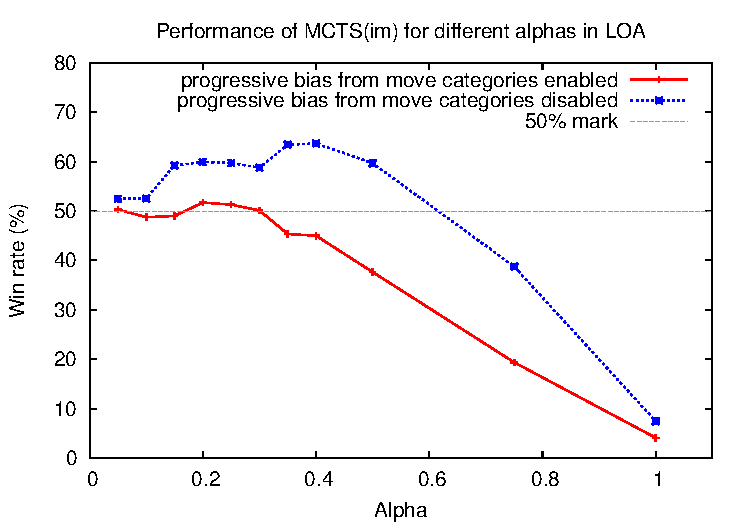
\includegraphics[scale=0.7]{plots/loa-alpha}
\caption{Results in LOA. Each data point represents 1000 games with 1 second of search time.} 
\label{fig:loa-alpha}
\end{center}
\end{figure}

\bibliographystyle{aaai}
\bibliography{im-mcts}


\end{document}
